\section{Timing and coordinate errors at the crossing event}
\label{app:event}

\subsection{Closed-form control and event projection}
With a fixed launch position and readings at \(h\) and \(2h\), the constant-acceleration interpolant uses
\begin{equation}
 \widehat{\vv a}=\frac{\vv r_2-2\vv r_1+\vv r_0}{h^2},
 \qquad
 \widehat{\vv v}_0=\frac{\vv r_1-\vv r_0}{h}
                         -\frac{h}{2}\widehat{\vv a}.
\end{equation}
For the prescribed readings this yields \((30.4,9.4,6.9)\) m/s and
\((-16,-16,-12)\) m/s\(^2\). This is a kinematic diagnostic. It assumes constant acceleration beyond the observations. Write \(X=11-x_0\), \(D=v_{0x}^2+2a_x X\), and assume a positive, transversal first forward root. A numerically stable evaluation is
\begin{equation}
 T=\frac{2X}{v_{0x}+\sqrt{D}},\quad
 \dot{x}(T)=\sqrt{D}.
\end{equation}
The nominal values are \(T=0.4050\) s and \((Y,Z)=(2.495,1.920)\) m. Equation~\eqref{eq:region} is obtained from the aerodynamic inference rather than this control.

Suppose an input perturbation changes the interpolated curve at fixed \(T\) by
\(\delta\vv r(T)\). Differentiating the event condition \(x(T)=11\) gives
\begin{equation}
 \delta T=-\frac{\delta x(T)}{\dot{x}(T)},\qquad
 \delta Q=P\,\delta\vv r(T),\qquad
 P=\begin{pmatrix}
 -\dot y(T)/\dot x(T)&1&0\\
 -\dot z(T)/\dot x(T)&0&1
 \end{pmatrix}.
 \label{eq:event-project}
\end{equation}
This expression converts longitudinal errors into lateral and vertical errors by the local slope of the path. A perturbation parallel to the local velocity changes the time to first order and cancels out of \(Q\). Near \(\dot x(T)=0\) the derivative can grow without bound, and when the forward root disappears the linearized location is undefined.

Let \(s=T/h\), \(\lambda_1=s(2-s)\), and \(\lambda_2=s(s-1)/2\). These are the Lagrange weights of the two observed positions when the launch anchor is fixed. With spatial errors \(\vv e_i\) and a shared true time shift \(\tau\) relative to the time labels, the first-order event shift is
\begin{equation}
 \delta Q=P\left[\lambda_1\vv e_1+\lambda_2\vv e_2+
        \bigl(\lambda_1\vv v(h)+\lambda_2\vv v(2h)\bigr)\tau\right].
 \label{eq:timing-spatial}
\end{equation}
At the nominal root the weights are \(-49.41\) and \(28.76\). Independent 5 mm per-axis bounds contribute first-order shifts of at most 0.439 m in \(Y\) and 0.424 m in \(Z\). A common 1 ms offset contributes \((-0.123,-0.093)\) m for positive offset under the stated sign convention. Central differences at \(1\,\mu\)s reproduce the timing derivative to within \(2\times10^{-5}\) m/s. The large values characterize extrapolation by an unconstrained quadratic. The main model restricts curvature through force and launch ranges.

\subsection{Joint perturbations and loss of a forward root}
For each timing bound and spatial bound, evaluate both phase endpoints and zero phase, and the corners of the six-coordinate box. A zero bound uses one value rather than repeating identical inputs. Refit the polynomial and solve the forward plane event for each case. Ground and goal-edge events are disabled in this diagnostic to isolate the existence of a forward plane root. The maximum shift is taken over tested roots only. A nonlinear map can attain its extrema away from the sampled corners, so this maximum is a scenario statistic.

\begin{table}[htbp]\centering\small
\caption{Joint timing and position stress test for the quadratic control. First-order maxima are coordinatewise sums of absolute derivative contributions. The sampled maximum is a Euclidean shift at a forward plane root. Counts include all selected timing and spatial combinations.}
\label{tab:plane-sens}
\begin{tabular}{@{}rrrrrr@{}}\toprule
Phase bound & Spatial bound & First-order \(Y\) & First-order \(Z\) & Sampled shift & No root\\
(ms) & (mm) & (m) & (m) & (m) & (count)\\\midrule
\csname @@input\endcsname tables/plane-sensitivity.tex
\bottomrule\end{tabular}
\end{table}

The quadratic can lose its plane crossing at a 3 ms timing bound. At 1 ms and 5 mm, all 192 combinations cross and the largest sampled displacement is 0.930 m. The corresponding coordinatewise linear bounds are 0.562 and 0.517 m. Larger perturbations change the root substantially, making the local derivative a poor global description. The different failure counts across spatial bounds reflect the changing discrete corners, not a monotone probability of failure. This is a reason to carry event uncertainty through the solver when propagating input uncertainty. A fixed-time error band alone cannot represent event loss.

\begin{figure}[htbp]\centering
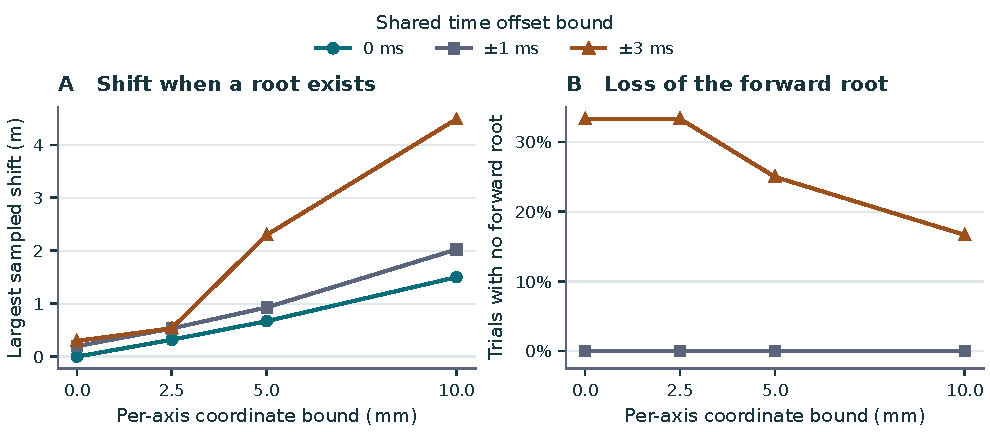
\includegraphics[width=\linewidth]{event-sensitivity.pdf}
\caption{\textbf{Input perturbations can move or remove the forward crossing.} A measures the maximum displacement among sampled corners with a root in the quadratic control. B reports the fraction of enumerated combinations without a root. These are deterministic trial fractions for the stated timing endpoints and position corners. The diagnostic considers the plane alone.}
\label{fig:event-shift}
\end{figure}

\subsection{Covariance propagation for correlated measurements}
Under independent coordinate noise with covariance \(\Sigma_e\) in each frame, a shared bias covariance \(\Sigma_b\), and an independent phase variance \(\sigma_\tau^2\), write \(w=\lambda_1\vv v(h)+\lambda_2\vv v(2h)\). The first-order covariance is
\begin{equation}
 \operatorname{Cov}(\delta Q)=
 P\left[(\lambda_1^2+\lambda_2^2)\Sigma_e+
        (\lambda_1+\lambda_2)^2\Sigma_b+
        \sigma_\tau^2 ww^\top\right]P^\top.
\end{equation}
The timing contribution is rank one. Its direction depends on the trajectory and event geometry. If a common coordinate translation were applied to release and frames alike, its effect would differ because the launch position would also change. The model uses an independently specified launch position. This formula separates local measurement amplification from model discrepancy and Monte Carlo variability. It is valid for a smooth forward crossing away from event switches.

\section{Operating points, subgroups and timing records}
\label{app:operating}
The operating points below report sample counts instead of treating calibration targets as test guarantees. Mean area includes every true direct entry. At a target of one the entire rectangular opening is returned by construction.

\begin{table}[htbp]\centering\small
\caption{Selected calibration targets and realized results from the 120-kick holdout. Rounded and tracking profiles share the 71 true direct entries.}
\label{tab:coverage-full}
\begin{tabular}{@{}llrrr@{}}\toprule
Profile & Forecast & Target (\%) & Hits & Mean area (m\(^2\))\\\midrule
\csname @@input\endcsname tables/coverage-targets.tex
\bottomrule\end{tabular}
\end{table}

\begin{table}[htbp]\centering\small
\caption{Hits at the 90\% calibration target by generator family and distance to the opening edge. The two edge strata partition direct entries. The three family strata form a separate partition. They are descriptive and were not separately calibrated.}
\label{tab:subgroup}
\begin{tabular}{@{}llrrrr@{}}\toprule
Profile & Stratum & Entries & 100 ms & 50 + 100 ms & Gravity\\\midrule
\csname @@input\endcsname tables/coverage-strata.tex
\bottomrule\end{tabular}
\end{table}

Near-edge means the minimum distance from the true direct entry to any of the four edges is below 0.244 m, the nominal cell width. The strata expose whether a successful overall average masks failures near the physical decision boundary. Family is available for evaluation only. The predictor never receives the synthetic truth label.

\begin{table}[htbp]\centering\small
\caption{Numerical availability and wall-clock timing in a single local run. Runtime includes inference and construction of the predicted region ranking inputs. The ballistic timing covers its trajectory result. Threshold application is omitted in both. Times are descriptive for this host and software environment.}
\label{tab:runtime}
\begin{tabular}{@{}llrrrrr@{}}\toprule
Profile & Forecast & Points & Events & ESS \(<25\) & Median (ms) & 95th (ms)\\\midrule
\csname @@input\endcsname tables/coverage-runtime.tex
\bottomrule\end{tabular}
\end{table}

The benchmark has one seed for each shot and profile. Paired intervals use 4,000 resamples of differences matched by shot ID. Event intervals use all shots. Position, area and hit intervals use the true direct entries. The test is balanced by generator family before observing outcomes. Intervals are descriptive of the sampled mixture. An independent field calibration would need known release, independent reference crossings, and an explicit protocol for intervening contacts.

\section{Implementation and physical checks}
\label{app:algorithm}
\subsection{A callable forecast contract}
The general method accepts the release point, a list of observed positions and timestamps, a camera-error model, and documented parameter supports. Input indices must be valid and coordinates finite. The solver advances each hypothesis from release to the last observation, rejecting a path that contacts the ground before the observations. Integrate surviving hypotheses until the earliest goal-plane crossing, descending ground contact, or horizon. The goal-plane coordinates are attached to an entry only when they lie in the open goal rectangle.

\begin{enumerate}
\item For each force family, sample wind and spin parameters. Form a launch-velocity proposal around the inversion of the last observation. Keep a 2\% prior draw to provide support away from the local proposal.
\item Evaluate the observation likelihood at all supplied times and assign importance weights as in Eq.~\eqref{eq:weights}. If including a timing nuisance, distribute the fixed budget over quadrature nodes and combine their masses with the node weights.
\item Carry posterior mass to first events. For each crossing through the goal, assign its weight to a fixed cell. Normalize the event masses using the total weight and normalize goal-cell masses using the entry weight.
\item Return the event vector, modal cell, raw region and effective sample size. Report an unavailable event distribution when total mass is zero. If total mass is positive but entry mass is zero, report the event distribution and mark the conditional point and map undefined.
\end{enumerate}

This separation avoids conflating a missed goal with an unsupported forecast. A boundary case can have a computed event vector and very little entry mass, so a conditional point should be accompanied by the unconditional entry probability. The physical support test and the numerical ESS warning answer separate questions.

\subsection{Model assumptions and checks}
\begin{table}[htbp]\centering\small
\caption{Roles of inputs in the nominal prediction. Changes to scenario choices require a fresh forecast.}
\label{tab:assumptions}
\begin{tabular}{@{}p{.31\linewidth}p{.24\linewidth}p{.36\linewidth}@{}}\toprule
Quantity & Role & Interpretation\\\midrule
Release, frame times, and opening & Given by the problem & Geometry and information budget\\
Ball mass, radius and air density & Nominal physical inputs & Set acceleration through the area-to-mass factor\\
Empirical drag curve & Literature-guided law & Limited range, with clipping and an offset prior\\
Wind and lift/spin bounds & Scenario and prior choices & Control admissible continuations and model weights\\
5 mm coordinate interval & Nominal rounding assumption & Relates reported positions to continuous paths\\
Cell resolution and RK4 steps & Numerical choices & Check stability before quoting modal coordinates\\
6 mm noise and 8 mm bias & Synthetic test parameters & Specify a noisy measurement regime\\
\bottomrule\end{tabular}
\end{table}

In the no-drag, no-lift limit, \(x(t)=v_{0x}t\), \(y(t)=v_{0y}t\), and \(z(t)=R+v_{0z}t-gt^2/2\). This gives closed-form plane and ground times and checks event ordering in the integrator. Under still-air drag without lift, both horizontal acceleration components are proportional to the corresponding velocity components, so the horizontal heading remains fixed. The constant-wind criterion in Eq.~\eqref{eq:wind} generalizes this relation in the wind frame. These limits check geometry and force signs independently of the posterior sampling.

For numerical cross-checks, the existing RK4 comparisons against adaptive DOP853 cover vacuum, drag with ground contact, effective lift and the speed-dependent empirical law. The largest reported event-position difference is 0.171 mm and the largest event-time difference is 0.038 ms. These four checks establish local numerical agreement under specified force laws. A finer solver cannot identify unknown wind, spin, or release-time error. The witness pair uses its own high-accuracy integration and a separate MATLAB replay.
